\documentclass[11pt]{article}
\usepackage{latexsym}
\usepackage{amsmath}
\usepackage{amssymb}
\usepackage{amsthm}
\usepackage{epsfig}
\usepackage{algpseudocode}
\usepackage{float} 
\usepackage[tight]{subfigure}

\usepackage{amsmath}
\usepackage{hyperref}

\DeclareMathOperator*{\minimize}{min}
\DeclareMathOperator*{\maximize}{max}

\usepackage{algorithm}
 %on linux you may need to run sudo apt-get install texlive-full to install algorithm.sys
\usepackage{algorithmic}

\usepackage{verbatim}

\newcommand{\handout}[5]{
  \noindent
  \begin{center}
  \framebox{
    \vbox{
      \hbox to 5.78in { {#1} \hfill #2 }
      \vspace{4mm}
      \hbox to 5.78in { {\Large \hfill #5  \hfill} }
      \vspace{2mm}
      \hbox to 5.78in { {\em #3 \hfill #4} }
    }
  }
  \end{center}
  \vspace*{4mm}
}

\newcommand{\lecture}[5]{\handout{#1}{#2}{#3}{#4}{#5}}
\newcommand{\collision}[0]{\mathrm{collision}}
\newcommand{\nocollision}[0]{\overline{\collision}}

\newcommand*{\QED}{\hfill\ensuremath{\square}}

\newtheorem{theorem}{Theorem}
\newtheorem{corollary}[theorem]{Corollary}
\newtheorem{lemma}[theorem]{Lemma}
\newtheorem{observation}[theorem]{Observation}
\newtheorem{proposition}[theorem]{Proposition}
\newtheorem{definition}[theorem]{Definition}
\newtheorem{claim}[theorem]{Claim}
\newtheorem{fact}[theorem]{Fact}
\newtheorem{assumption}[theorem]{Assumption}
\newtheorem{note}[theorem]{Note}

% 1-inch margins, from fullpage.sty by H.Partl, Version 2, Dec. 15, 1988.
\topmargin 0pt
\advance \topmargin by -\headheight
\advance \topmargin by -\headsep
\textheight 8.9in
\oddsidemargin 0pt
\evensidemargin \oddsidemargin
\marginparwidth 0.5in
\textwidth 6.5in

\parindent 0in
\parskip 1.5ex
%\renewcommand{\baselinestretch}{1.25}

\begin{document}

\lecture{Statistical Techniques in Robotics (16-831, S22)}{Lecture \#11
  (Monday, February 23)}{Lecturer: Kris Kitani}{Scribes: Yimin Tang, Zilin Si}{AdaBoost \& Multi-Armed Bandit}

\section{Review}
In the last lecture, we had learnt the online techniques applied on supervised learning, especially focused on online Support Vector Machine (SVM). 
\subsection{Hyperplanes}
In geometry, a hyperplane is a subspace whose dimension is one less than that of its ambient space. For example, if a space is 3-dimensional then its hyperplanes are the 2-dimensional planes, while if the space is 2-dimensional, its hyperplanes are the 1-dimensional lines\footnote{\href{https://en.wikipedia.org/wiki/Hyperplane#:~:text=In\%20geometry\%2C\%20a\%20hyperplane\%20is,are\%20the\%201\%2Ddimensional\%20lines}{Wikipedia}}.

Taken the hyperplanes (lines) in 2D as example, it can be written as $w_1 x_1 + w_2 x_2 + b = 0$, and in the vector form, $\textbf{w} \cdot \textbf{x} + b = 0$, where $\textbf{w} \in \mathbb{R}^2$. Alternatively, we can merge the bias term $b$ into the weight vector $\textbf{w}$ such that $ \textbf{w} \cdot \textbf{x} = 0$, where $\textbf{w} \in \mathbb{R}^3$. 

\paragraph{Distance to origin}: Given a line $\textbf{w} \cdot \textbf{x} + b = 0$, the distance from the line to the origin is $\rho = \frac{b}{||\textbf{w}||}$.
\paragraph{Distance between two parallel lines}: Given a line $\textbf{w} \cdot \textbf{x} + b = 0$ and another parallel line $\textbf{w} \cdot \textbf{x} + b = -1$, the distance in between is $\rho = \frac{b+1}{||\textbf{w}||} - \frac{b}{||\textbf{w}||} = \frac{1}{||\textbf{w}||}$.

Similarly, the hyperplanes of 3D are planes, and we can represent them as $\textbf{w} \cdot \textbf{x} + b = 0$, where the distance from the plane to the origin is $\frac{b}{||\textbf{w}||}$. And given two planes $\textbf{w} \cdot \textbf{x} + b = 1$ and $\textbf{w} \cdot \textbf{x} + b = -1$, the distance in between is $\rho =\frac{b+1}{||\textbf{w}||} - \frac{b-1}{||\textbf{w}||} = \frac{2}{||\textbf{w}||}$

\subsection{Support Vector Machine and max-margin classification}
Support Vector Machine (SVM)~\cite{noble2006support} can be used as a max-margin classifier. It aims to separate the data given the labels by finding a hyperplane that can maximize the margin between data groups. And this maximum margin solution is most stable to perturbations of data. Assume the hyperplane with maximum margin is $\textbf{w} \cdot \textbf{x} + b = 0$, and the inner points are locating at the boudary of margin $\textbf{w} \cdot \textbf{x} + b = 1$ and $\textbf{w} \cdot \textbf{x} + b = -1$. Then the objection is to maximze the margin:\newpage
\begin{equation}
    max_{\textbf{w}} \frac{2}{||\textbf{w}||}
\end{equation}
subject to $\textbf{w} \cdot \textbf{x}_i + b$ is $\geq 1$ if $y_i = 1$ or $\leq -1$ if $y_i = -1$ for all $i$.

This problem is equivalent to 
\begin{equation}
    min_{\textbf{w}} ||\textbf{w}||
\end{equation}
subject to $y_i (\textbf{w}\cdot \textbf{x}_i + b) \geq 1$ for all $i$. 

And this is a convex quadratic programming (QP) problem where a unique solution exists.

However, due to the noise or non-separability of the data, it may not be possible to satisfy all constraints. Here we introduce the soft margin SVM which allows some misclassification to get more robust classification by using a slack variable $\xi$:
\begin{equation}
    y_i (\textbf{w} \cdot \textbf{x}_i + b) \geq 1 - \xi_i
\end{equation}
Geometrically, the slack $x_i$ is the distance from the misclassified point $\textbf{x}_i$ to the margin.

Now the problem becomes
\begin{equation}
    min_{w,\xi} ||\textbf{w}||^2 + C \sum_{i} \xi_i
\end{equation}
subject to $y_i (\textbf{w}\cdot \textbf{x}_i + b) \geq 1 - \xi_i$ for all $i$.

And to merge the linear constraints into the objective function, this becomes
\begin{equation}
    min_{w} (\frac{\lambda}{2}||\textbf{w}||^2 + \frac{1}{M} \sum_{m=1}^{M} 1 - y_m \textbf{w}^T \textbf{x}_m)
\end{equation}

However, we only want to penalize for mistakes, weakly correct but ignore the very correct data, we replace the contraints term with a hinge loss and it turns to
\begin{equation}
     min_{w} (\frac{\lambda}{2}||\textbf{w}||^2 + \frac{1}{M} \sum_{m=1}^{M} max\{0, 1 - y_m \textbf{w}^T \textbf{x}_m\})
\end{equation}

Now this problem is convex with linear loss fuction $max\{0, 1 - y_m \textbf{w}^T \textbf{x}_m\}$ and quadratic regularization $\frac{\lambda}{2}||\textbf{w}||^2$, but it is non differentiable due to the hinge.
To solve this problem, we use stochastic (Sub) gradient descent for linear SVMs.

\subsection{Online sub-gradient descent (OMD)}
For the hinge loss $max\{0, 1 - y_m \textbf{w}^T \textbf{x}_m\}$, there are many possible sub-gradients, but we use two sub-gradients:

\begin{equation}
  \textbf{z}_m =
    \begin{cases}
      \textbf{0} & \text{if $y_m \textbf{w}^T \textbf{x}_m \geq 1$}\\
      -y_m \textbf{x}_m & \text{otherwise}
    \end{cases}       
\end{equation}

Till here, we can write the soft SVM algorithm as 

\begin{algorithm}
\caption{soft SVM}
\begin{algorithmic}[1]

\State $\theta^{(1)} \leftarrow 0 \in \mathbb{R}^N$
    \For{$t=1...T$}
        \State $y_d, x_d \sim D$
        \State $\theta^{(t)} = \theta^{(t-1)} + y_d x_d \cdot 1[y_d (\textbf{w}^{(t)} \cdot \textbf{x}_d) < 1]$
        \State $\textbf{w}^{(t+1)} \leftarrow \frac{1}{\lambda (t+1)\theta^{(t)}}$
    \EndFor
\State $\bar{\textbf{w}} = \frac{1}{T} \sum_{t} \textbf{w}^t$

\end{algorithmic}
\end{algorithm}


\section{Summary}

\subsection{PAC Learning Model}

A Probably Approximately Correct(PAC)~\cite{valiant1984theory} learning algorithm requires :

\begin{equation}
E_{p(x, y)}[\mathbf{1}[f(x ; \mathcal{D}) \neq y]]<\epsilon
\end{equation}

holds with probability $1-\delta $ for any dataset $D$ with size $N$ drawn from true distribution $P(x,y)$.

There are two types of PAC Learning Models, one is strong PAC-learning algorithm, the other is weak PAC-learning algorithm:
\begin{itemize}
    \item \textbf{Strong PAC-learning algorithm}: Given $\epsilon, \delta$ and $\mathcal{D} \sim P(x, y)$,
learner outputs with probability ($1-\delta$) a hypothesis with error at most $\epsilon$. And run-time must be polynomial in $\frac{1}{\delta}$ and $\frac{1}{\epsilon}$  and other relevant parameters such as the size of the examples or complexity of the target concept.
    \item \textbf{Weak PAC-learning algorithm}: We can release the error to $\epsilon \geq 1 / 2-\gamma$. And any weak learning algorithm can be boosted into a strong learning algorithm.
\end{itemize}


\subsection{AdaBoost}

We can call a weak PAC learner multiple times (generates a sequence of hypothesis) but present
it with a different distribution at each time, then combine all hypothesis into a single learner, this learner can be a strong PAC learner. 

For example, we have a binary classification problem. We can get an strong classifier by combining weighted weak learner.
\begin{figure}[htbp]
    \centering
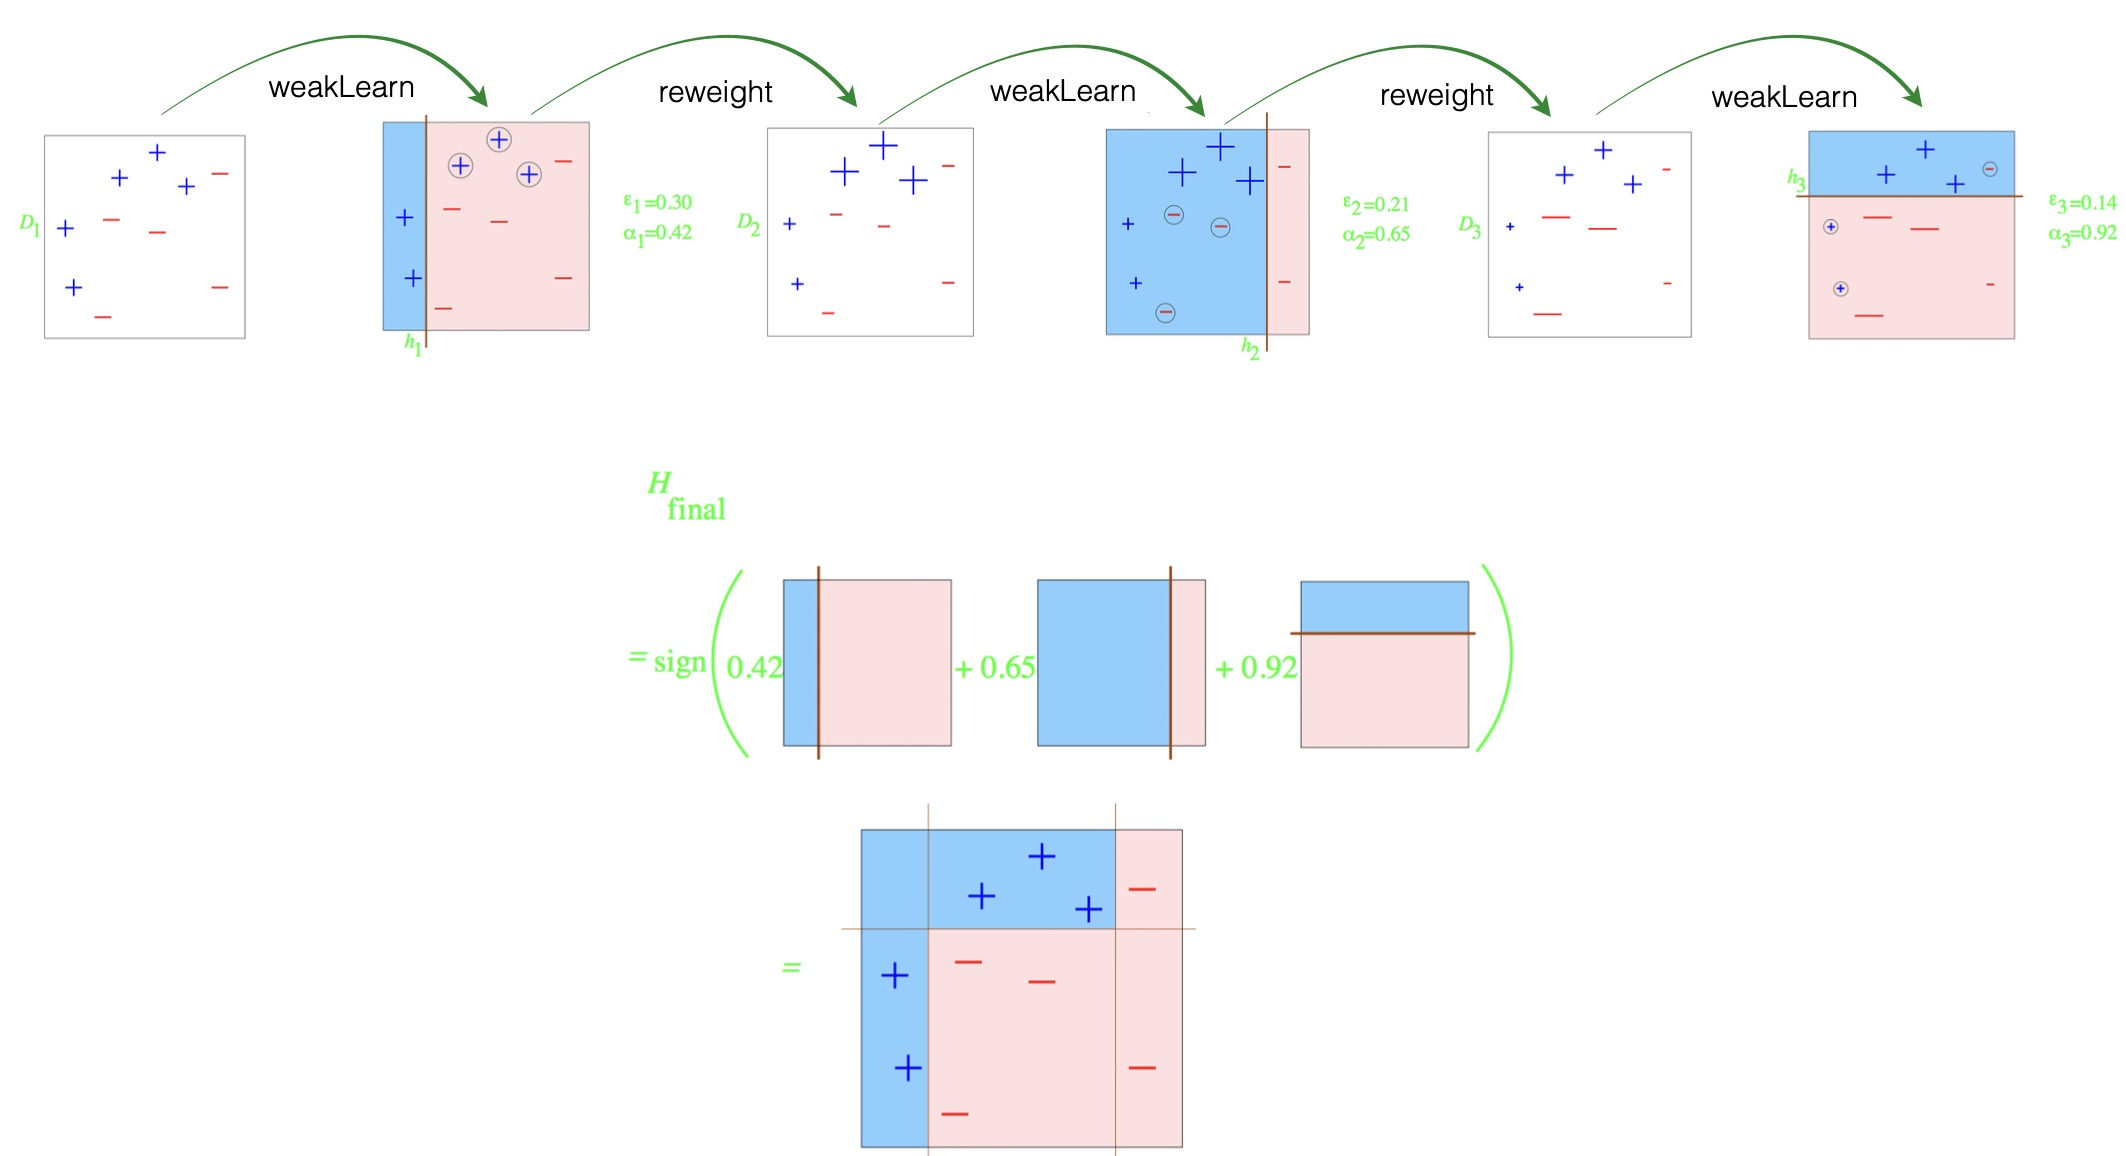
\includegraphics[width=15cm]{0D45E115-583C-4075-948D-8CB24B907D8E.png}
    \caption{Toy example}
    \label{fig:galaxy}
\end{figure} 

\begin{algorithm}
\caption{Adaboost}
\begin{algorithmic}[1]

\Function{Adaboost}{$\boldsymbol{D}=\left\{\boldsymbol{x}_{n}, y_{n}\right\}_{n=1}^{N},\left\{w_{n}^{(0)}\right\}_{n=1}^{N}, T$}
    \For{$t=1...T$}
        \State $\boldsymbol{p}^{(t)}=\boldsymbol{w}^{(t-1)} / \sum_{n} w_{n}^{(t-1)}$
        \State $h^{(t)}=$ WEAKLEARNER $\left(\boldsymbol{D}, \boldsymbol{p}^{(t)}\right)$ \Comment{Prediction}
        \State $\epsilon^{(t)}=\sum_{n} p_{n}^{t}\left|h^{(t)}\left(x_{n}\right)-y_{n}\right|$
        \State $\beta^{(t)}=\epsilon^{(t)} / 1-\epsilon^{(t)}$
        \State $w_{n}^{(t)}=w_{n}^{(t-1)} \beta^{1-\left|h^{(t)}\left(\boldsymbol{x}_{n}^{(t)}\right)-y_{n}^{(t)}\right|} \forall n$ \Comment{Update}
    \EndFor

\end{algorithmic}
\end{algorithm}

The final error bound is: 
\begin{equation}
    \epsilon \leq 2^{T} \prod_{t=1}^{T} \sqrt{\epsilon_{t}\left(1-\epsilon_{t}\right)}
\end{equation}

The main difference between WMA and Adaboost is changing weights over experts versus data. And Adaboost will learn one weak learner with re-weighting dataset, WMA just re-weighting the experts and selects one.

\subsection{Multi-Armed Bandit}

\subsubsection{Overview}

\begin{figure}[htbp]
    \centering
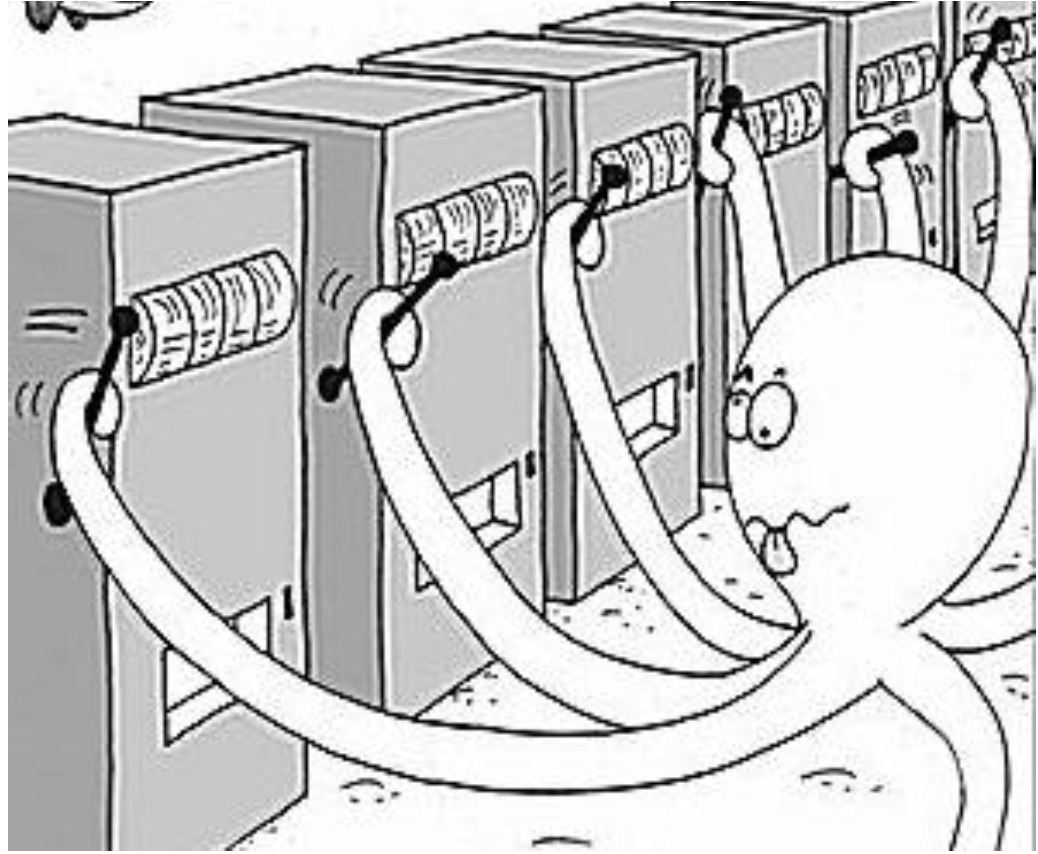
\includegraphics[width=10cm]{83BC5798-A361-4DFB-AB9E-C6E591FFE33A.png}
    \caption{Multi-armed bandit problem}
    \label{fig:bandit}
\end{figure} 

In the multi-armed bandit problem settings, we have multiple bandits with unknown reward distribution. Each time we are allowed to pull one arm and get this bandit's reward. Without knowing other bandits' rewards in each iteration, we should use learning strategies to maximize our total rewards over $T$ iterations based on our historical information. \\



There could be different types of observations in this learning problem:
\begin{itemize}
    \item \textbf{one-shot feedback}: In each time step, we only perform one action and get one reward. This action won't change the state of the next time step.
    \item \textbf{exhaustive feedback}: Since states and actions are finite, the player can pull all arms over the duration of the game. 
    \item \textbf{evaluative feedback}: The player receives a sampled reward from the underlying reward distribution at each time step.
\end{itemize}

\subsubsection{PWEA vs Bandits}
PWEA and MAB problems both target to maximize the rewards or minimize the regrets, however they are different in the problem settings.

For PWEA, the player can get access to all experts' losses after taking an action so that he can remove or down-weight experts at each time step. However, for MAB, the player can only get access to the loss of the expert that's been selected. Mathematically, the player chooses an action $a^{(t)} \in \{1,2, ..., n\}$ at time step $t$, then for PWEA, the player observes loss vector for all possible actions as $l^{(t)}\in [0,1]^N$; but for MAB, the player can only observe loss for his action as $l^{(t)}_{a^{(t)}}\in [0,1]$.


\subsubsection{Exploration and Exploitation Trade-off}

Since with MAB, the player only gets to see the rewards of the arm pulled, we need to find the balance between 1) exploiting arms that did well in the past and 2) exploring arms that might do well in the future. This doesn't apply to PWEA because it will explore automatically as the player can see all rewards.

\subsubsection{Applications}
Some applications of MAB are:
\begin{itemize}
    \item \textbf{A/B testing}: The searching engine displays advertisements and gets rewards from the user who clicks ads.
    \item \textbf{Robot grasping}: The robot learns to grasp with different strategies with the reward as it can successfully pick up the object.
    \item \textbf{Medical treatment}: The doctor gives medicines to the patient where the reward is the patient gets healthy.
    \item \textbf{Packet routing}: The data packet is sent to a target location along a path where the reward comes from the low round-trip time.
    \item \textbf{AI for Go}: The algorithm explores the space of the future actions and gets win as a reward.
\end{itemize}
All these applications can only explore one action at each time step and get this action's reward.

\subsubsection{Stochastic Bandit}
For stochastic bandit~\cite{robbins1952some}, each arm has its own static reward distribution and each pulls gives the player a sample from this distribution. In order to maximize the rewards in a certain $T$ rounds, the player has to consider the exploration-exploitation trade-off.

Mathematically, we assume each arm $k$ has a static reward distribution as $v_k(r)$ with mean $\mu_k$. By pulling, we sample a reward $r^{(t)}$ from this distribution. 

Give multiple arms $k = 1, 2, ..., N$ with reward distribution $v_1(r), v_2(r), ..., v_N(r)$ and mean $\mu_1, \mu_2, ..., \mu_N$, to maximize the rewards, the player should pull the arm with the highest mean. However, during the game, the player does not know the true distribution and mean of each arm but only knows the estimated mean $\hat{\mu_1}^{(t)}, \hat{\mu_2}^{(t)}, ..., \hat{\mu_N}^{(t)}$ after number of pulls $T_1(t), T_2(t), ..., T_N(t)$. Therefore it is hard to choose which arm to pull to maximize the rewards because there might be difference between the estimated and the true mean.



%\section*{References}
%Include your references here. Please cite any resources you found useful.	
%Populate the refs.bib file or list your references manually. Be consistent in formatting!
{
\bibliography{refs}
\bibliographystyle{abbrv}
}

%\section{Appendix}
%This section provides any relevant background material that was not covered in the lectures, but was found to be useful for understanding the material. 
%For example, derivations, theory underlying techniques employed, etc. 

%Additionally, this section can summarizes applications or extensions of these techniques found in the literature. 

\end{document} % Done!


